\documentclass[11pt]{article}
\pdfinfoomitdate=1\pdftrailerid{}
\usepackage[letterpaper,margin=.7in,headheight=15pt,headsep=18pt,footskip=24pt]{geometry}
\usepackage[T1]{fontenc}\usepackage{lmodern,amsmath,amssymb,array,booktabs,fancyhdr,hyperref,tikz}
\usetikzlibrary{arrows.meta}
\renewcommand{\familydefault}{\sfdefault}\setlength{\parindent}{0pt}\setlength{\parskip}{7pt}
\pagestyle{fancy}\fancyhf{}\fancyhead[L]{\small Week NN / Hidden armies / Facilitator guide}
\fancyfoot[L]{\scriptsize Bellingham Math Circle / Week NN / HA-FAC-v1}\fancyfoot[R]{\thepage}
\hypersetup{hidelinks}
\newcommand{\head}[1]{\par\textbf{\large #1}\par}
\newcommand{\sub}[1]{\par\textbf{#1}\par}
% side view of a hill mat: hills at x0, x0+1.3, x0+2.6; towers of cubes; tokens on hills won
\newcommand{\mat}[6]{% x0, y0, h1, h2, h3, token list
  \foreach \i/\n in {0/#3,1/#4,2/#5}{%
    \draw[line width=.7pt,fill=black!4] ({#1+1.3*\i},#2) ellipse (.5 and .16);
    \node[font=\scriptsize\bfseries] at ({#1+1.3*\i},{#2-.4}) {\the\numexpr\i+1\relax};
    \ifnum\n>0 \foreach \k in {1,...,\n}{%
      \draw[line width=.5pt,fill=black!25] ({#1+1.3*\i-.15},{#2+.3*(\k-1)}) rectangle ({#1+1.3*\i+.15},{#2+.3*\k});}\fi}
  \foreach \t in {#6}{\ifnum\t>0 \fill ({#1+1.3*(\t-1)+.36},{#2-.02}) circle (.11);\fi}}
\newcommand{\strp}[5]{% x, y, three numbers
  \foreach \i/\v in {0/#3,1/#4,2/#5}{%
    \draw[line width=.6pt] ({#1+.55*\i},#2) rectangle ({#1+.55*(\i+1)},{#2+.5});
    \node at ({#1+.55*\i+.275},{#2+.25}) {\v};}}
\begin{document}
\head{Mathematical overview: no plan is safe, and beating goes round in circles}
\textbf{The game.} Each player secretly splits the same number $N$ of cubes over hills 1, 2 and 3 (a hill may stay empty), written hill by hill as in 3-0-2. A hill goes to the taller tower, an equal hill to nobody, and more hills wins. There are $(N+1)(N+2)/2$ plans: 21 with 5 cubes, 28 with 6. With equal armies a game ties exactly when some hill is equal (the other two then hold equal totals, so they split or both tie); otherwise it ends 2 hills to 1. Rearranging the hills of both plans alike never changes a result, so only a plan's \emph{type} matters (1-4-1 has type 4-1-1).

\textbf{Theorem 1: the cheapest win.} Let a plan have hills $a\ge b\ge c$ with $a\ge1$. The fewest cubes that beat it is $b+c+2$: one more than it on each of its two smaller hills and nothing on its biggest. \emph{Proof.} A winner wins more hills than it loses. Winning two hills needs one more than the plan on each of them, and the two smaller hills are cheapest, at $b+c+2$. Winning one hill and tying the other two costs $a+b+c+1\ge b+c+2$. Extra cubes never spoil a win, so every larger army can also win. (The empty plan 0-0-0 is beaten by 1 cube.)

\textbf{Theorem 2: from 4 cubes on, no plan is safe.} With equal armies a plan can be beaten exactly when $b+c+2\le N$, that is, when its biggest hill holds at least 2 cubes. The \emph{counter-plan} puts one more than the partner on each of the two smaller hills and the remaining $a-2$ on the biggest; it wins two hills whatever happens on the third. From 4 cubes on some hill holds 2 or more (three hills of at most 1 hold at most 3), so every plan can be beaten. The plans nobody can beat are exactly those with no hill above 1: every plan with 1 cube; 1-1-0, 1-0-1 and 0-1-1 with 2; and 1-1-1 alone with 3. In children's terms: taking a hill from 1-1-1 costs 2 cubes and leaves 1 for the other two.

\textbf{Theorem 3: ranking the 28 six-cube plans.} Every plan with $N$ cubes ties exactly $2N+1$ plans, itself included: 13 of the 28 with 6 cubes, so ``beats'' plus ``is beaten by'' is always $28-13=15$. \emph{Why:} a tie needs an equal hill; $N+1-p_i$ plans match $p$ on hill $i$, $2N+3$ in all, and matching on two hills forces the whole plan, so subtract 3 and add 1 back. Number of plans each beats, by type: 6-0-0 none, 5-1-0 5, 4-2-0 8, 4-1-1 and 3-3-0 9, 3-2-1 11, 2-2-2 12 (the 28 counts total 210). So 2-2-2 beats the most, yet 3-3-0, 3-0-3 and 0-3-3 beat it: taking two of its hills costs $3+3$ cubes, and taking one while tying two costs 7. And 6-0-0 beats nothing: it can win only hill 1, and then the partner wins hill 2 or hill 3. Beating the most plans is not being unbeatable.

\textbf{Theorem 4: circles.} Beating is not transitive: 0-1-5 beats 2-0-4, which beats 1-2-3, which beats 0-1-5. With 6 cubes there are 180 circles of three plans, each counted once. Every plan except 6-0-0, 0-6-0 and 0-0-6 lies on one: the circles 2-2-2 $\to$ 4-1-1 $\to$ 3-3-0 and 0-2-4 $\to$ 3-1-2 $\to$ 1-5-0 meet the six other types, and rearranging the hills of all three plans in a circle gives another circle. A plan that beats nothing cannot be on a circle.

\textbf{Unpredictability (adult remark; Grades 4--5 Problem 8).} Since from 4 cubes on every fixed plan can be beaten, good play has to be unpredictable; Borel (1921) began the theory of such games with this idea. Rolling a die to choose among the six arrangements of 4-2-0 cannot be exploited: no 6-cube plan beats more of those six than it loses to. The game is symmetric, so no way of playing guarantees more than an even score on average; this die guarantees at least that (and wins on average against 6-0-0), so it is a best possible way to play. The six arrangements of 3-2-1 are exploited by 3-3-0, which beats two and loses to none.

\textbf{Limits and evidence.} Everything assumes three hills, whole cubes, a majority of hills and equal hills to nobody; points per hill, more hills or a tie-break change the answers. Theorems 1, 2 and the tie count are proved for every $N$; the 6-cube counts, circles and dice are exhaustive computer checks (\texttt{check\_guide.py}). For children, not finding a safe plan is an experiment, ``no plan is safe'' a conjecture, and the counter-plan the explanation from 4 cubes on. Fewest-cubes rows suggest $b+c+2$; Theorem 1 proves it. A full 28-plan table settles only 6 cubes.

\textbf{What each band does.} \emph{K--1} (5 cubes, pictures; an adult reads): play; test plans against a partner; find safe plans with 2 and 3 cubes, none with 4 or 5; meet a best plan and a circle; beat plans with fewest cubes; find every plan that beats a given one. \emph{Grades 2--3} (6 cubes, strips): hunt for a safe plan; beat any named plan and say how; see why 1-1-1 is safe and no 4-cube plan is; build circles, none with 6-0-0; make complete lists; find the fewest-cubes rule. \emph{Grades 4--5}: explain the counter-plan for any size; find which sizes have a safe plan; rank the 28 plans; find which lie on circles; prove the fewest-cubes rule; compare unequal armies; test plans chosen by dice.
\newpage
\head{Preparation, launch and pacing}
\textbf{Status.} Draft for the organizer's review; unpiloted. Nothing has been tried with real materials: building plans behind standing folders, sliding one hill mat above another to compare, K--1 children drawing on the printed boards, the time the pooled Grades 4--5 table takes and the preparation time are all untested.

\textbf{Prerequisites.} K--1 needs counting to 5 and comparing two towers; children need not read, since the adult reads each problem. Grades 2--3 read short problems, write a plan as three numbers and add small numbers. Grades 4--5 also organize many cases and explain why a method always works. Grade labels are rough: K--1 Problem 7 asks the same kind of question as Grades 2--3 Problem 6, and Grades 2--3 Problem 7 the same kind as Grades 4--5 Problem 6, which adds 40-30-30 and asks why the rule works.

\textbf{Materials for the current group (4 K--1, 4 Grades 2--3, 3 Grades 4--5).} \emph{Hill mats:} materials p.~1, ``Hill mat'', two mats to a sheet; one mat per child and one per launch adult, 13 mats from 7 sheets. \emph{Cubes} of one colour, interlocking (about 2~cm) so towers survive being moved: 6 per K--1 child and 10 per older child, about 100 in all, plus 14 for the launch. Older children build at most 10 each (the 10-cube rows of Grades 2--3 Problems 3 and 7 and Grades 4--5 Problem 2); plans of 20 or 100 cubes are written, not built. \emph{A file folder} per child and per launch adult. \emph{Win tokens} that look different from the cubes, such as pennies: three per pair. Pencils. A die for Grades 4--5 Problem 8 is optional; the problem needs none.
\begin{center}\small
\begin{tabular}{@{}lcccc@{}}
\toprule
 & Materials p.~1 sheets & Cubes & Folders & Tokens\\
\midrule
K--1 table (4 children) & 2 & 24 & 4 & 6\\
Grades 2--3 table (4) & 2 & 40 & 4 & 6\\
Grades 4--5 table (3) & 2 (one mat spare) & 30 & 3 & 6\\
Launch (2 adults) & 1 & 14 & 2 & 3\\
\bottomrule
\end{tabular}
\end{center}

\textbf{Printing and preparation.} Print single-sided on US Letter at 100\%: the K--1 packet (6 pages) four times, Grades 2--3 (5 pages) four times, Grades 4--5 (6 pages) three times plus one extra page 3 as the shared table, and materials p.~1 seven times, on card stock if you have it. The materials footer has a 100~mm scale bar; if it measures 10~cm, the hills are the intended 7~cm across. Cut each materials sheet once, along its dashed line, into two mats. Nothing else is cut or made by hand; children draw (K--1) or write (older bands) in their own packets. Allow about 20 minutes for printing, cutting the 7 sheets and bagging cubes and tokens by table, plus 5 minutes for the two launch adults to rehearse. This estimate is untested.

\textbf{Seating, screens and comparing.} Seat partners side by side, so both read hills 1, 2, 3 from left to right; the mats do not work across a table, where the hills face each other in the wrong order. Folders are needed only for hidden games: K--1 Problem 1, Grades 2--3 Problem 1 and the opening games of Grades 4--5 Problem 1. For those, stand the opened folders upright between the two mats, like a wall. Later problems show plans openly. To compare, one partner slides a mat directly above the other's, so the grey bands line up and hill 1 sits above hill 1, as in the K--1 rules picture. Whether towers survive the slide, and whether children line up the bands without help, is untested; if towers topple, compare by pointing hill by hill.

\textbf{Staffing.} One adult per table. \emph{K--1 (parent volunteer):} read each problem aloud, keep the hide--lift--compare rhythm, let children place the tokens, and draw for a child who asks. Do not choose plans or say whether a plan can be beaten. When a child claims a plan nobody can beat, ask the partner to try, then the other pair at the table. If nobody beats it, you may take one turn as challenger and build a beating plan from the key below; the children check it hill by hill, so the game gives the verdict, not you. If time runs out first, take the claim to the sharing minutes or keep it for the return visit, and record it. \emph{Grades 2--3:} read as needed, check that each strip matches its towers, and handle a ``safe plan'' claim the same way. \emph{Grades 4--5:} in hidden games the third child referees, rotating; help the children split the shared table. Reading and recording are ordinary adult support; if the adult is choosing the plans, return to building with cubes.

\textbf{Launch (about 5 minutes, after running around).} Give each child cubes, a hill mat and a folder for a minute of free building. Then two adults sit side by side, with the children gathered behind them so that everyone reads hills 1, 2, 3 from left to right, and play with 7 cubes each (7, so that no launch plan, even rearranged, appears on any page).

\emph{Game 1.} Adult A builds 5-0-2 and Adult B builds 4-3-0, behind a folder wall. Lift the folders together and slide B's mat above A's. Ask the children, hill by hill, who has more. A puts tokens on hills 1 and 3, B on hill 2. A wins, 2 hills to 1.

\emph{Game 2.} B says, ``I'll try to beat your last plan,'' and builds 2-0-5. But A has changed to 2-5-0. Hill 1 is equal, so nobody takes a token; A wins hill 2 and B wins hill 3. One hill each: a tie. Say once: ``Both players may change their plan every game.''

For the older tables, write Game 1 on the board as two strips labelled A and B, reading hills 1, 2, 3, and circle the winner. Do not discuss which plans are good; that is what the tables find out.
\begin{center}
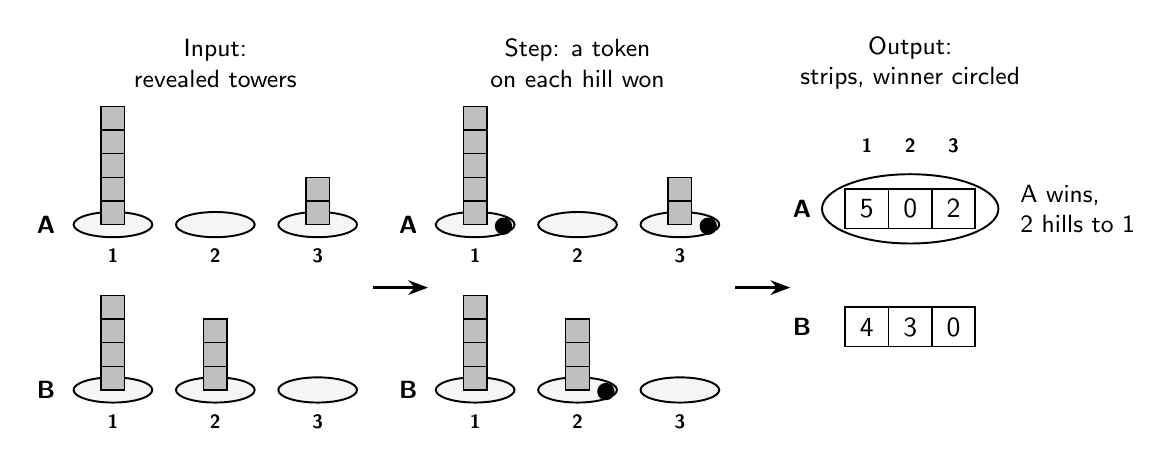
\begin{tikzpicture}
\node[font=\small,align=center] at (1.3,4.15) {Input:\\revealed towers};
\node[font=\small\bfseries] at (-.85,2.1) {A};\node[font=\small\bfseries] at (-.85,0) {B};
\mat{0}{2.1}{5}{0}{2}{0}
\mat{0}{0}{4}{3}{0}{0}
\draw[-{Stealth[length=2.5mm]},line width=.8pt] (3.3,1.3) -- (4.0,1.3);
\node[font=\small,align=center] at (5.9,4.15) {Step: a token\\on each hill won};
\node[font=\small\bfseries] at (3.75,2.1) {A};\node[font=\small\bfseries] at (3.75,0) {B};
\mat{4.6}{2.1}{5}{0}{2}{1,3}
\mat{4.6}{0}{4}{3}{0}{2}
\draw[-{Stealth[length=2.5mm]},line width=.8pt] (7.9,1.3) -- (8.6,1.3);
\node[font=\small,align=center] at (10.125,4.15) {Output:\\strips, winner circled};
\foreach \i in {1,2,3}{\node[font=\scriptsize\bfseries] at ({9.3+.55*\i-.275},3.1) {\i};}
\node[font=\small\bfseries] at (8.75,2.3) {A};
\strp{9.3}{2.05}{5}{0}{2}
\draw[line width=.7pt] (10.125,2.3) ellipse (1.12 and .44);
\node[font=\small\bfseries] at (8.75,.8) {B};
\strp{9.3}{.55}{4}{3}{0}
\node[font=\small,anchor=west,align=left] at (11.4,2.3) {A wins,\\2 hills to 1};
\end{tikzpicture}
\end{center}

\textbf{A first hour and later visits.} Table work is 35--40 minutes. \emph{K--1:} Problem 1 (about 10 minutes of play), Problem 2 (about 15), then Problem 3. Return visit: Problems 4 and 5, then 6 and 7. \emph{Grades 2--3:} Problem 1 (about 10 minutes; it can stop after four or five games), Problem 2 (10--15), Problem 3 (about 15), and Problem 4 for quick pairs. Return visit: Problems 5 and 6, then 7. \emph{Grades 4--5:} Problem 1 (about 10), Problems 2 and 3 (about 20), then Problem 6, which extends Problem 2's idea, or a start on Problem 4. Return visit: Problems 4 and 5 together, then 7, with Problem 8 last; quick children can take the four-hill question under Problem 3. Finishing every page is not the goal. For the sharing minutes, ask each table: ``Did anyone find a plan nobody could beat?''

\head{Grades K--1 (packet HA-K-v1)}
Plans are built on the hill mats (materials p.~1) and written hill 1, hill 2, hill 3; read 2-1-2 aloud as ``2 on hill 1, 1 on hill 2, 2 on hill 3.'' On the printed boards children draw a plan as squares stacked on the hills; when Problem 2's boards first come up, point to the towers in the rules picture on page 1. A dot or a numeral for each hill is fine.

\sub{Problem 1, page 1: play with 5 cubes}
Each child builds on a hill mat behind the folder wall. Watch for children comparing totals, which are always equal, instead of hill by hill, and for a child who claims the game because of one tall tower. Many games tie, since any equal hill makes a tie. Hint: ``Point to hill 1. Who has more there?''

\sub{Problem 2, page 1: is there a plan with 5 cubes that nobody can beat?}
No: every 5-cube plan loses to some plan. The hardest to beat are 2-2-1, 2-1-2 and 1-2-2, each beaten by only 2 of the 21 plans: 2-2-1 by 3-0-2 and 0-3-2, 2-1-2 by 3-2-0 and 0-2-3, 1-2-2 by 2-3-0 and 2-0-3. Expect a pair to believe they have found a safe plan; the next step is the partner trying, not the adult saying, then the steps under Staffing. A child's explanation with cubes: ``I put one more than you on your two short towers.'' Hint, only for a stuck pair: ``Which hill could you let your partner have?''

\sub{Problem 3, page 2: draw a plan with 5 cubes that beats each plan}
One plan per row; children may build the printed plan on one mat and try a beater on the other. Complete lists, for checking: 5-0-0 loses to the 10 plans with at least 1 cube on both hill 2 and hill 3, such as 1-2-2 or 3-1-1; 0-4-1 to 3-0-2, 2-1-2, 2-0-3, 1-2-2, 1-1-3 and 1-0-4; 0-3-2 to 2-0-3, 1-4-0, 1-1-3 and 1-0-4; 2-1-2 only to 3-2-0 and 0-2-3. The rows get harder, and the last is hard. Hint: ``Which two hills will you win?''

\sub{Problem 4, page 3: 2 cubes? 3 cubes? 4 cubes?}
2 cubes: yes, one cube on each of two hills (1-1-0, 1-0-1 or 0-1-1); taking a hill from it uses both cubes. 3 cubes: yes, 1-1-1 only. 4 cubes: no. Each row has one board, so the 4-cube board may end up holding a plan the children think is safe, most likely 2-1-1, 1-2-1 or 1-1-2, each beaten by just one plan (2-1-1 by 0-2-2). Ask the partner to try with cubes, then follow the steps under Staffing. Follow-up for children who found 1-1-1: ``How do you know nobody can beat it?''

\sub{Problem 5, page 4: is one plan the best?}
Partners each build one plan of a row on a mat. Each box holds three plans, each in its own column and each met twice. Top box, rows from the top: 2-2-1 beats 4-1-0, 2-2-1 beats 0-0-5, and 4-1-0 beats 0-0-5. So 2-2-1 won both its games and is the best in this box. Bottom box: 0-1-4 beats 2-0-3, 2-0-3 beats 1-2-2, and 1-2-2 beats 0-1-4. Each plan wins once and loses once: there is no best plan, and the three go round in a circle. Hint: ``Which plan won both of its games?'' Extension: lay the three bottom plans in a ring and point from each winner to the plan it beat.

\sub{Problem 6, page 5: beat each plan with as few cubes as you can}
5-0-0: 2 cubes (only 0-1-1). 1-4-0: 3 (only 2-0-1). 1-3-1: 4 (only 2-0-2). 2-2-1: 5 (3-0-2 or 0-3-2). 1-1-1: 4 (six ways, such as 2-2-0 or 2-1-1), more cubes than 1-1-1 has. The rule behind these (add the two shorter towers, then add 2) is for the adult; a child's reason is ``one more than each short tower, and nothing on the tall one.'' Hint: ``Do you need to win the tall tower?'' Follow-up: ``Could you do it with one cube fewer?''

\sub{Problem 7, page 6: every plan with 5 cubes that beats it}
3-1-1: exactly 3, namely 1-2-2, 0-3-2 and 0-2-3 (4 boards). 4-0-1: exactly 6, namely 2-1-2, 1-2-2, 1-1-3, 0-3-2, 0-2-3 and 0-1-4 (8 boards). Spare boards stay empty. Why the lists are complete: winning hill 1 from 4-0-1 takes all 5 cubes, and winning one hill while tying two takes 6, so a winner must take hills 2 and 3, with at least 1 cube on hill 2 and 2 on hill 3; going through 0, 1 and 2 cubes on hill 1 gives three, two and one plans. Against 3-1-1, winning hill 1 takes 4 cubes and leaves 1, which can at best tie one other hill, and winning one hill while tying two takes 6; so a winner needs at least 2 cubes on each of hills 2 and 3, leaving 0 or 1 for hill 1. Hint: ``How will you know when you have found them all?''

\head{Grades 2--3 (packet HA-23-v1)}
Plans are built on the hill mats (materials p.~1) whenever a game is played or a plan is tested, and recorded as strips.
\sub{Problem 1, page 1: play with 6 cubes and record}
Nearly half of all pairings of different 6-cube plans tie (168 of 378), so many games have no winner to circle; a game ties exactly when some hill is equal. Check that strips list hills 1, 2, 3 in order.

\sub{Problem 2, page 1: is there a plan with 6 cubes that nobody can beat?}
No; the counter-plan beats every plan. Expect children to settle on 2-2-2, which only 3-3-0, 3-0-3 and 0-3-3 beat, or on an arrangement of 3-2-1, which loses to 4 plans. Hint: ``Can you win two of its hills?''

\sub{Problem 3, page 2: beat each plan, then a way to beat any plan}
Counter-plans (other answers work too): 2-2-2 by 0-3-3; 1-4-1 by 2-2-2; 3-0-3 by 1-1-4; 0-1-5 by 1-2-3; 3-2-2 by 1-3-3; 1-1-5 by 2-2-3; 4-4-2 by 2-5-3; 2-5-3 by 3-3-4; 7-7-6 by 5-8-7. Check any answer hill by hill. The way: one more than the partner on each of the two smaller hills and the rest on the biggest, which wins those two hills. It works whenever the biggest hill has at least 2 cubes, which is always true from 4 cubes on. Hint: ``Which hill can you afford to lose?'' Follow-up: ``Are there always enough cubes left over?'' This leads into Problem 4.

\sub{Problem 4, page 2: 3 cubes, then 4}
1-1-1, with the explanation under Theorem 2: taking one of its hills costs 2 cubes and leaves 1 for the other two, so the best is a tie (3-0-0 even loses). With 4 cubes there is no such plan: every plan has a hill with at least 2 cubes, so Problem 3's way works. The hardest is 2-1-1, beaten only by 0-2-2.

\sub{Problem 5, page 3: circles of three plans}
The arrows run top $\to$ right $\to$ left $\to$ top, each plan beating the next. Any circle will do in the first two diagrams, such as top 0-1-5, right 2-0-4, left 1-2-3. With 2-2-2 on top: right 4-1-1, left 3-3-0. Twelve circles contain 2-2-2, and the left plan must be 3-3-0, 3-0-3 or 0-3-3, the only plans that beat 2-2-2. With 6-0-0 it cannot be done, because 6-0-0 beats no plan (Theorem 3), so no plan can follow it round a circle. Hints: ``What has to beat 2-2-2?'' and ``What does 6-0-0 beat?''

\sub{Problem 6, page 4: every plan that beats 2-2-2, then 6-0-0}
2-2-2 loses exactly to 3-3-0, 3-0-3 and 0-3-3 (6 strips are printed). There are no others: winning a hill of 2-2-2 costs 3, so winning two hills uses all 6 cubes and leaves the third hill empty, and winning one hill while tying two costs $3+2+2=7$. 6-0-0 loses exactly to the 15 plans with at least 1 cube on both hill 2 and hill 3 (20 strips): 0-1-5, 0-2-4, 0-3-3, 0-4-2, 0-5-1; 1-1-4, 1-2-3, 1-3-2, 1-4-1; 2-1-3, 2-2-2, 2-3-1; 3-1-2, 3-2-1; 4-1-1. A plan with nothing on hill 2 or hill 3 at best ties. Hint: ``Can you list them in an order that would show you a missing one?''

\sub{Problem 7, page 5: beat each plan with as few cubes as you can}
6-0-0: 2 (0-1-1). 4-1-1: 4 (0-2-2). 3-2-1: 5 (0-3-2). 2-2-2: 6 (3-3-0). 3-3-0: 5 (4-0-1). 1-1-1: 4 (2-2-0), more than the partner's 3. 8-1-1: 4 (0-2-2). 5-3-2: 7 (0-4-3). The quick way: add the two smaller hills, then add 2 (Theorem 1, whose proof a child can give in words). Hint: ``Do you need to win all three hills? Which two?'' Extension: ``Which 6-cube plan needs the most cubes to beat?'' (2-2-2, with 6.)

\head{Grades 4--5 (packet HA-45-v1)}
\sub{Problem 1, page 1: is there a plan with 6 cubes that nobody can beat?}
As Grades 2--3 Problem 2: no. Plans are built on the hill mats (materials p.~1). In the opening hidden games two children play and the third referees; for testing, one shows a plan and the other two try to beat it; rotate.

\sub{Problem 2, page 2: beat each plan, then a way for any plan with 6 or more cubes}
Counter-plans: 2-2-2 by 0-3-3; 1-4-1 by 2-2-2; 3-2-2 by 1-3-3; 1-1-5 by 2-2-3; 3-3-3 by 1-4-4; 1-8-1 by 2-6-2; 7-7-6 by 5-8-7; 34-33-33 by 32-34-34; 50-0-50 by 48-1-51 (or 0-1-99, among others). The way and its explanation are Theorem 2's counter-plan; it needs a biggest hill of at least 2, true of every plan from 4 cubes on. Hint for the 100-cube rows: ``Which two hills will you win, and by how much?''

\sub{Problem 3, page 2: for which numbers of cubes is there a plan nobody can beat?}
Exactly 1, 2 and 3 (and trivially 0): Theorem 2, with Problem 2's way as the counter-plan. The safe plans are 1-1-1 with 3 cubes, 1-1-0 and its arrangements with 2, and any plan with 1, where every game ties. Hint: ``When does your Problem 2 way run out of cubes?'' Extension for quick children, with plans written as four or five numbers: ``What if there are 4 hills, or 5, with the same rules?'' A plan nobody can beat exists exactly when there are no more cubes than hills, and the safe plans are those with no hill above 1. The counter-plan still works on any plan with a hill of 2 or more: give up the biggest hill, put one more on two other hills and match the rest. A plan with no hill above 1 is safe: a challenger has only as many cubes as the plan has 1-hills, but pays 2 for each 1-hill won and 1 for each empty hill won, so for each hill won some 1-hill is left empty and lost. (Checked for 4 hills up to 12 cubes and 5 hills up to 10.)

\sub{Problem 4, page 3: how many of the 28 plans each plan beats}
Counts: 0 for 6-0-0, 0-6-0, 0-0-6; 5 for each arrangement of 5-1-0; 8 for each arrangement of 4-2-0; 9 for 4-1-1, 1-4-1, 1-1-4 and for 3-3-0, 3-0-3, 0-3-3; 11 for each arrangement of 3-2-1; 12 for 2-2-2. Most: 2-2-2. Fewest: the three all-on-one-hill plans. Rearranged plans get the same count, so only seven plans need full work. Leave that discovery to the children and hold ``Do 4-1-1 and 1-4-1 have to get the same count?'' in reserve. Without it the table is 378 games; with it, at most 189 (7 plans against 27 others). Each game gives a result for both plans in it. Checks: the counts total 210, and each plan's ``beats'' and ``beaten by'' add to 15. The table can fill most of a session; pool it and stop when the pattern is clear.

\sub{Problem 5, page 4: which plans can be part of a circle?}
Every plan except 6-0-0, 0-6-0 and 0-0-6. The circles 2-2-2 $\to$ 4-1-1 $\to$ 3-3-0 and 0-2-4 $\to$ 3-1-2 $\to$ 1-5-0 meet all six other types, and rearranging the hills of all three plans in a circle gives another circle, which reaches every arrangement. A plan that beats nothing cannot be followed round a circle. Hint: ``If 4-1-1 is on a circle, must 1-4-1 be on one too?''

\sub{Problem 6, page 5: the fewest cubes, and a rule}
6-0-0: 2 (0-1-1). 4-1-1: 4 (0-2-2). 3-2-1: 5 (0-3-2). 2-2-2: 6 (3-3-0). 1-1-1: 4 (2-2-0). 40-30-30: 62 (0-31-31); no 61-cube plan beats it. Rule and proof: Theorem 1. Expect children to skip its second case, winning one hill and tying two; ask ``Could you win just one hill and still win the game?''

\sub{Problem 7, page 5: against a partner with 6 cubes}
8 cubes for a plan the partner cannot beat: exactly 3-3-2, 3-2-3 and 2-3-3. 9 for a plan that beats every 6-cube plan: only 3-3-3. \emph{Proof for 8.} By Theorem 1, 6 cubes beat your plan $x\ge y\ge z$ exactly when $y+z+2\le6$. So safety needs $y+z\ge5$, hence $y\ge3$ and $x\ge3$, and the total is at least 8, with 8 only for 3-3-2. \emph{Proof for 9.} Against any plan of at most 9 cubes except 3-3-3, the partner puts one more than your smallest hill there and the rest on your middle hill. Your two smaller hills total at most 5 (a total of 6 or more within at most 9 cubes forces every hill to hold 3, which is 3-3-3), so the partner wins one hill and ties or wins another. And 3-3-3 beats everything: a partner can top 3 on at most one hill, since $4+4>6$, leaving at most 2 cubes for the other two hills; a partner who tops no hill wins nothing and has some hill below 3. The answers stay the same if the partner may also use fewer cubes. Hint: ``What would your partner do against your plan?''

\sub{Problem 8, page 6: Ben's and Mia's dice}
Ben: 3-3-0, 3-0-3 or 0-3-3, each beating two of his six plans, tying four and losing none. Mia: there is none. Her list holds every arrangement of 4-2-0, so a plan and its rearrangements score alike against her, and one plan of each of the seven types covers all 28. Wins and losses against her six plans: 6-0-0, 0 and 2; 4-2-0, 1 and 1; 2-2-2, 0 and 0; and 2 and 2 for each of 5-1-0, 4-1-1, 3-3-0 and 3-2-1. Nobody does better than break even against Mia; since the game is symmetric nobody can guarantee more, so her die is a best possible way to play (overview). Hint: ``Against Mia, does it matter which arrangement of a plan you test?'' Follow-up: ``2-2-2 breaks even against both Ben and Mia. Is playing 2-2-2 every time as good as Mia's die?'' (No: once your partner knows it, 3-3-0 beats it.)

\head{Sources, connections and use}
Émile Borel, ``La théorie du jeu et les équations intégrales à noyau symétrique'', \emph{Comptes Rendus de l'Académie des Sciences} 173 (1921): the allocation game and the idea of mixing plans. Brian Roberson, ``The Colonel Blotto game'', \emph{Economic Theory} 29 (2006), 1--24: the general continuous game. Both are cited from the theme outline; neither was consulted for this guide. Competitive Kids, ``Blotto'', \url{https://www.competitivekids.org/games/blotto}: as the outline reports it (accessed October 24, 2026), a classroom version with 100 soldiers on 3 to 7 fronts that also reports ``every fixed plan has a counter''. The page could not be reached from this environment and was not re-consulted for this guide. The small cube armies, the proofs of Theorems 1--4, the ranking by plans beaten and the two dice are this theme's own; \texttt{check\_guide.py} recomputes every answer above from the final pages.

Connections named in the outline (not re-read for this guide): Week 24's decks beat each other in a circle, Week 87's majority rankings cycle, atlas AP-22 builds a randomizer a rival cannot exploit, and Week 58 divides goods fairly. New here: a simultaneous allocation game, the counter-plan argument, and ranking plans by how many they beat.

After a session, record which problems each table reached; whether K--1 compared hill by hill without help; any plan a table believed nobody could beat, and how they found out; whether towers survived sliding the mats and children lined up the grey bands without help; how long the shared table took; and what children wanted to continue.

\end{document}
